\documentclass[conference]{IEEEtran}
\usepackage{todonotes}
%\todo{Make a cake}
\usepackage{url}
\usepackage{lipsum}
% Basically, \url{my_url_here}.

% *** CITATION PACKAGES ***
%
\usepackage{cite}
% \cite{} output to follow that of the IEEE.
% The documentation is contained in the cite.sty file itself.

% *** MATH PACKAGES ***
%
%\usepackage{amsmath}
% A popular package from the American Mathematical Society that provides
% many useful and powerful commands for dealing with mathematics.
%
% Note that the amsmath package sets \interdisplaylinepenalty to 10000
% thus preventing page breaks from occurring within multiline equations. Use:
%\interdisplaylinepenalty=2500
% after loading amsmath to restore such page breaks as IEEEtran.cls normally
% does. amsmath.sty is already installed on most LaTeX systems. The latest
% version and documentation can be obtained at:
% http://www.ctan.org/pkg/amsmath

% *** ALIGNMENT PACKAGES ***
\usepackage{array}
\usepackage{tikz,tabularx,amsthm,amsmath,amssymb,amsfonts,listings,xcolor,enumerate,url,array,
	multirow,forest}

% *** SUBFIGURE PACKAGES ***
%\ifCLASSOPTIONcompsoc
%  \usepackage[caption=false,font=normalsize,labelfont=sf,textfont=sf]{subfig}
%\else
%  \usepackage[caption=false,font=footnotesize]{subfig}
%\fi
% subfig.sty, written by Steven Douglas Cochran, is the modern replacement
% for subfigure.sty, the latter of which is no longer maintained and is
% incompatible with some LaTeX packages including fixltx2e. However,
% subfig.sty requires and automatically loads Axel Sommerfeldt's caption.sty
% which will override IEEEtran.cls' handling of captions and this will result
% in non-IEEE style figure/table captions. To prevent this problem, be sure
% and invoke subfig.sty's "caption=false" package option (available since
% subfig.sty version 1.3, 2005/06/28) as this is will preserve IEEEtran.cls
% handling of captions.
% Note that the Computer Society format requires a larger sans serif font
% than the serif footnote size font used in traditional IEEE formatting
% and thus the need to invoke different subfig.sty package options depending
% on whether compsoc mode has been enabled.
%
% The latest version and documentation of subfig.sty can be obtained at:
% http://www.ctan.org/pkg/subfig


% *** Do not adjust lengths that control margins, column widths, etc. ***
% *** Do not use packages that alter fonts (such as pslatex).         ***
% There should be no need to do such things with IEEEtran.cls V1.6 and later.
% (Unless specifically asked to do so by the journal or conference you plan
% to submit to, of course. )


% correct bad hyphenation here
\hyphenation{op-tical net-works semi-conduc-tor}


\begin{document}
%
% paper title
% Titles are generally capitalized except for words such as a, an, and, as,
% at, but, by, for, in, nor, of, on, or, the, to and up, which are usually
% not capitalized unless they are the first or last word of the title.
% Linebreaks \\ can be used within to get better formatting as desired.
% Do not put math or special symbols in the title.
\title{Title of the article}


% author names and affiliations
% use a multiple column layout for up to three different
% affiliations
\author{\IEEEauthorblockN{Mahieddine Yaker\\ and Julien Cartigny \\and Gilles Grimaud}
\IEEEauthorblockA{IRCICA\\
University of Lille\\
address in Lille\\
Email: yyy@yyy.com}
\and
\IEEEauthorblockN{Chrystel Gaber \\ and Xiao Han \\ and Vicente Sanchez-Leighton}
\IEEEauthorblockA{Orange Labs,\\
Ch\^{a}tillon, France\\
Email: firstname.lastname@orange.com\\}
}

% conference papers do not typically use \thanks and this command
% is locked out in conference mode. If really needed, such as for
% the acknowledgment of grants, issue a \IEEEoverridecommandlockouts
% after \documentclass

% for over three affiliations, or if they all won't fit within the width
% of the page, use this alternative format:
% 
%\author{\IEEEauthorblockN{Michael Shell\IEEEauthorrefmark{1},
%Homer Simpson\IEEEauthorrefmark{2},
%James Kirk\IEEEauthorrefmark{3}, 
%Montgomery Scott\IEEEauthorrefmark{3} and
%Eldon Tyrell\IEEEauthorrefmark{4}}
%\IEEEauthorblockA{\IEEEauthorrefmark{1}School of Electrical and Computer Engineering\\
%Georgia Institute of Technology,
%Atlanta, Georgia 30332--0250\\ Email: see http://www.michaelshell.org/contact.html}
%\IEEEauthorblockA{\IEEEauthorrefmark{2}Twentieth Century Fox, Springfield, USA\\
%Email: homer@thesimpsons.com}
%\IEEEauthorblockA{\IEEEauthorrefmark{3}Starfleet Academy, San Francisco, California 96678-2391\\
%Telephone: (800) 555--1212, Fax: (888) 555--1212}
%\IEEEauthorblockA{\IEEEauthorrefmark{4}Tyrell Inc., 123 Replicant Street, Los Angeles, California 90210--4321}}

% make the title area
\maketitle

% As a general rule, do not put math, special symbols or citations
% in the abstract
\begin{abstract}
Abstract \todo[inline]{TBD}
%%\lipsum[1]
\end{abstract}

% no keywords




% For peer review papers, you can put extra information on the cover
% page as needed:
% \ifCLASSOPTIONpeerreview
% \begin{center} \bfseries EDICS Category: 3-BBND \end{center}
% \fi
%
% For peerreview papers, this IEEEtran command inserts a page break and
% creates the second title. It will be ignored for other modes.
\IEEEpeerreviewmaketitle



\section{Introduction}
\label{sec:Intro}
% no \IEEEPARstart
%\todo[inline]{TBD}


Internet of things (IoT) devices and cyber-physicals systems (CPS) are becoming ubiquitous in our modern society\cite{WOlf2018}. IoT is in the interest of many industrials issuer. We can see an increase of devices including multiples hardware and software components in order to provide more complex services\cite{Xu2014}.

In that kind of environment, privacy, safety and security issues for the end-users are becoming one of the main concern of the industrial. Moreover, in one device, we can identify a certain number of distinct industrial entities which provide software and hardware services for the end-user. The IoT device is becoming a competitive environment where each service provider may have to trust in economic competitors.


By considering the importance of trust between industrial entities, we propose in this paper a platform architecture and design based on a separation kernel and a communication mechanism control to guarantee for each service provider a trustworthy environment.

This paper is structured as follow, section \ref{sec:IoTissue} describes a simple security issue into household IoT. In section \ref{sec:Isolation_model} we are going to introduce Pip, a separation kernel which provides a proved memory isolation mechanism. Section \ref{sec:Industrial_ecosystem} describes the industrial ecosystem and the responsibilite of each actor. In Section \ref{sec:Architecture}, we can find the ODSI architecture in details and in section \ref{sec:illustration_discussion} we can see how to build a real industrial example with Pip and the ODSI platform.
%\lipsum[1-2]
%\hfill mds
 
%\hfill March 05, 2018


\section{Internet of Things security issues}
\label{sec:IoTissue}
Oravec and co \cite{Oravec2017} described in their paper the increase of utilization of devices and applications dedicated to Internet of Things, particularly in the case of household appliances and house management. They wished to demonstrated the new issues that should be considered with the expansion of IoT into the house. One of their main concern is the security and privacy integrity of users. They descried scenario about different attacks or other information due to fallible household devices and non-secure softwares. 

In that kind of environment, Sivaraman and co\cite{Sivaraman2016} described a scenario based on an attack on all house IoT devices via a smartphone application. By using the smartphone and network accesses into the house, they found all available IoT devices. In their paper, they show how it is possible to get control of each device. With this attack, they show that even if there is strong network security mechanisms (like router equipped with firewalls) if any component of the House IoT has an application level issue, the security and privacy is no more guaranteed into the house. This attack works with a smartphone, but we can also imagine a scenario where an another connected device (Webcam, connected TV..) can be an attack vector. 


In the past years, security and privacy was one of the main concern of the academic and industrial researchs\cite{BernalBernabe2016}\cite{Xu2014}\cite{Razzaque2016}. They have designed different architecture models in order to provide more trustworthy environments for the IoT industrial and the end-users.


\section{Isolation model}
\label{sec:Isolation_model}
%\todo[inline]{TBD by Lille}
%\lipsum[1-10]
\subsection{Memory isolation proto-kernel}

\begin{figure}
	\centering
	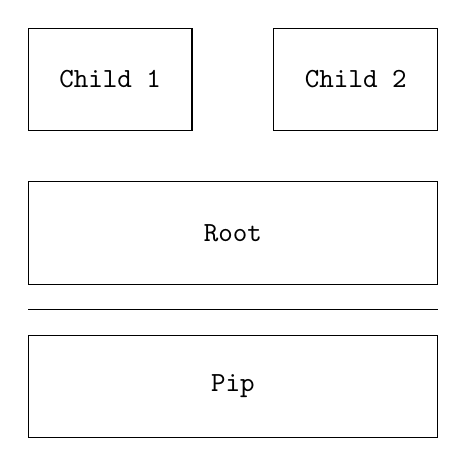
\begin{tikzpicture}[baseline=0, scale=2.6]
	% Draw rectangles
	\draw(-1, -2) rectangle (1, -1.5);
	\draw(-1, -1.25) rectangle (1, -0.75);
	\draw(-1, -0.5) rectangle (-0.2, 0);
	\draw(0.2, -0.5) rectangle (1, 0);
	
	% Draw kernel-user separation
	\draw[-] (-1,-1.375) -- (1, -1.375);
	
	% Draw text
	\draw (0,-1.75) node{\texttt{Pip}} ;
	\draw (0,-1) node{\texttt{Root}} ;
	\draw (-0.6,-0.25) node{\texttt{Child 1}} ;
	\draw (0.6,-0.25) node{\texttt{Child 2}} ;
	\end{tikzpicture}
	\caption{Pip architecture view} 
	\label{fig:PipArchBase}
\end{figure}



PIP\cite{bergougnoux2017} is a protokernel: it allows for kernels, ranging from hypervisors to monolithic kernels, to be developed as user mode applications (figure \ref{fig:PipArchBase}). This means that only PIP is executed in kernel mode (i.e., the privileged mode of the hardware)(figure . Indeed, code running in kernel mode has direct access to the whole memory and hardware. It is thus clearly better, from a security point of view, to keep this code as minimal as possible. This stems from the general principle that the trusted computing base (TCB) should be kept minimal. One of the PIP key design is to have a minimal number of functionalities while ensuring strong isolation. More precisely, PIP only manages memory isolation and redirection of interruptions to user space code, and has only 10 system calls. Contrary to micro-kernel, it means that components like scheduler, IPC and authorization are not included in the PIP kernel, neither other mechanism available in monolithic kernel like device abstraction layer, file systems, network stack, etc.



\begin{figure}[h!]
	%	\begin{minipage}[c]{5.1cm}
	%	\end{minipage}
	\hfill
	%	\begin{minipage}[c]{0.65\linewidth}
	
	\centering
	\begin{forest}
		for tree={grow=east,reversed,minimum height=0.7cm}
		[P$_{\mbox{root}}$
		[P$_1$
		[P$_{1.1}$
		[P$_{1.1.1}$]
		[P$_{1.1.2}$]
		[P$_{1.1.3}$]
		]
		[P$_{1.2}$
		[P$_{1.2.1}$]
		[P$_{1.2.2}$]
		]
		]
		[P$_2$
		[P$_{2.1}$]
		[P$_{2.2}$]
		]
		]
	\end{forest}
	\caption{The view by Pip of the partition tree}
	\label{abstree:fig}
	%	\end{minipage}
\end{figure}
PIP proposes a hierarchic  memory isolation model (figure \ref{abstree:fig}) to partition the available memory among several memory-limited space called partition. A partition is a set of physical memory pages mapped to virtual address. At start, all the available memory (as defined inside PIP configuration) makes up the ROOT partition. The root partition can include mapped registers from hardware devices, thus providing access to hardware functionalities. Code executed in a parent partition can request (via system calls to PIP) segregation to its memory space: a new child partition is created on which the parent partition can mapped a subset of its own mapped physical memory pages, thus \textit{delegating} part of its memory space to the child partition. This model is recursive: any partition can create a child partition and delegate part of its memory space. While a partition can read and write in the memory of its child partition (we call this property vertical sharing), sibling partitions cannot access each other's memory (we call this property horizontal isolation).
\subsection{Pip memory management}

\begin{figure}[h!]
	\centerline{\includegraphics[height=3.5cm]{figures/properties.eps}}
	\caption{Isolation model}
	\label{props:fig}
\end{figure}

Pip model ensure formal isolation between partitions. This isolation is guaranteed by two properties :


\begin{itemize}
	\item \textbf{Horizontal isolation} : Two distinct partitions (ex: \textit{child 1} and \textit{child 2} in figure \ref{props:fig}) can not share the same memory pages.
	\item \textbf{Vertical sharing} : All pages used by a child are mapped into its parent. 
\end{itemize}


As seen in figure \ref{props:fig}, for partition creation, a parent gives the required amount of memory pages from its own pages to its child, and theses pages belong to this new partition.

In order to create partition and manage each child memory, Pip provide a set a function available for each partition.
\begin{itemize}
	\item \textbf{createPartition} : create a new partition.
	\item \textbf{deletePartition} : delete a new partition.
	\item \textbf{addVAddr} : gives a page to a child partition (no more available into the parent).
	\item \textbf{removeVAddr} : reclaims a page from a child partition (no more available into the parent).
\end{itemize}


\subsection{Interrupt management}
To manage interruptions, PIP has two different behaviours depending of the kind of interruption:
\begin{itemize}
	\item Software interrupts (fault or system calls) are relayed to the parent partition (with the exception of the PIP system calls).
	\item Hardware interrupts are relayed to the ROOT partition which is in charge to forward it to, for instance, a network card driver.
\end{itemize}

Furthermore, a parent receives all software interruptions from its children%\footnote{With the notable exception of the PIP system calls, as a partition can create sub-partitions only based on a (sub)set of its own memory space, thus not breaking the hierarchic isolation model.}
, thus controlling which interactions have its children with the system.

In addition, Pip API provides two function for software interrupt between partitions :
\begin{itemize}
	\item \textbf{dispatch} : send an interrupt signal to a given partition.
	\item \textbf{resume} : restores a previous interrupted partition.
\end{itemize}

Any partition can send and receive a signal only from its parent, one of its child and from Pip. For example, in figure \ref{props:fig} There is no available signal transmission between \textit{p1} and \textit{p2} or \textit{p3} and \textit{p2}.


\subsection{IPC mechanism}
\begin{figure}[h!]
	\centering
	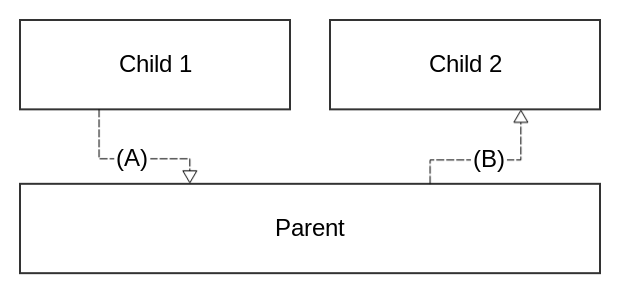
\includegraphics[width=0.7\linewidth]{figures/IPCDispatch}
	\caption{Simple IPC mechanism}
	\label{fig:ipcdispatch}
\end{figure}


Pip does not provide IPC between two distinct partitions. However, this mechanism can be implemented in userland, by using software interrupt or Pip API dispatch function. For example (figure \ref{fig:ipcdispatch}), if \textit{Child 1} wants to send a message to \textit{Child 2}, it has to send a dispatch to its \textit{parent} (step A). The parent handles this software interrupt and transmit the signal to \textit{Child 2} (step B).

For more complex architecture (like figure \ref{abstree:fig}), this mechanism can be recursively used to send signal between any partitions (ex : P1.1 to P.1.2.2).


\section{Industrial ecosystem}
\label{sec:Industrial_ecosystem}
This section describes the industrial ecosystem and the needs for a security architecture based on isolation. First, we identify and define the stakeholders involved in the use and management of an IOT or M2M device. The responsibilities of each actor are then described and finally, the requirements for an isolation-based architecture are listed.\\

We consider that a domain is an isolated area which belongs to an entity. The notion of domain is precised in section \ref{sec:Domain_def}.\\

We distinguish device ressources and domain ressources. Device ressources correspond to the isolated partitions (domains) and the ressources exposed by software, actuators or sensors drivers installed by the packager in the owner domain and which are related to the device. Domain ressources correspond to any ressource not related to the device and created within the given domain. En example of device ressource is the firmware or its updater. An example of a domain ressource is a key to create an SSL channel between a remote platform and a given domain.\\

\subsection{Actors}
\label{sec:Actors}
We identify 7 stakeholders, namely the manufacturer, packager, maintainer, owner, administrator, service provider and user, which interact with the IOT ot M2M device. One device may be associated to 1 packager, 1 owner, 1 administrator and several manufacturers, maintainers and service providers. One actor may hold several roles. For example, one actor can be at the same time a manufacturer, a packager and a maintainer.
\subsubsection{Manufacturer}
Manufacturers provide at least one component of the device, either a physical component with its driver, an operating system or an isolation solution. Manufacturers also provide updates \& patches for the component and the driver to the packager and/or maintainers. 
\subsubsection{Packager}
It issues the device and the isolation solution. It also provides each device an identifier that will subsequently allow it to be identified as well as intial secrets that will allow the owner to access the device. It may also provide the drivers and software components for the sensors or actuators on the device. 
\subsubsection{Maintainer}
It maintains the device, monitors the hardware components status and deploys the patches delivered by the manufacturer. 
\subsubsection{Owner}
The device belongs to the Owner who defines an access policy to authorize which other entities are authorized to use or manage the device or domains within the device. The Owner can possess several devices. It receives initial credentials from the manufacturer that allows it to access each device in his fleet. 
\subsubsection{Administrator}
It enforces the policy defined by the owner for his fleet of devices. If any modification, such as adding a new entity or modifying its granted permissions,  is required, it requests a decision from the owner. This role can either be assumed or delegated to a third party by the owner. 
\subsubsection{Service Provider}
It delivers a user-friendly service on one or multiple devices using the ressources authorized by the Owner. It installs or activates a service within the device. Muliple Service Providers can co-exist on the same device. 
\subsubsection{User}
Users consume the services provided by the entities mentioned above. We can distinguish platform users and technical users. Service users subscribe to the services provided by the Service Providers. Technical users are typically members of the Owner, Manufacturer, Maintainer entities and they will perform authorized administration actions such as creating a new domain, granting rights to a new user, loading a service on the device. In the rest of this article, we focus on platform users.
 
\subsection{Responsibilities model}
\label{sec:Resp_model}

The responsibilities described in this section are summarized in table \ref{tab:resp_table}.\\

\begin{table*}[!ht]
% increase table row spacing, adjust to taste
\renewcommand{\arraystretch}{1.3}
% if using array.sty, it might be a good idea to tweak the value of
% \extrarowheight as needed to properly center the text within the cells
\caption{Responsibilities matrix}
\label{tab:resp_table}
\centering
% Some packages, such as MDW tools, offer better commands for making tables
% than the plain LaTeX2e tabular which is used here.
\begin{tabular}{|p{7cm}||c|c|c|c|c|c|c|}
\hline
Responsibilities & Manufacturer & Packager & Maintainer & Owner & Administrator & Service Provider\\
\hline
Provide device components (hardware \& drviers, OS, isolation solution) & X & & & & &\\
\hline
Gather components into a device & & X & & & &\\
\hline
Use or provide virtualization \& multi-tenant compatible components & & X & & & &\\
\hline
Provide mechanisms \& temporary credentials for initial device personalization before delivery to the owner & & X & & & &\\
\hline
Provide temporary credentials for initial domain personalization to entities after delivery to the owner & & X & & X & X & \\
\hline
Update regularly the credentials to access its domain & & & X & X & X & X\\
\hline
Provide components or devices to owner without remote backdoor access & X & X & & & & \\
\hline
Create / Modify / Delete a domain before delivery to owner & & X & & & & \\
\hline
Create / Modify / Delete a domain after delivery to owner & & & & X & X & \\
\hline
Configure the access policy of the device ressources & & & & X & X & \\
\hline
Enforce the device ressource access policy & & & & X & X & \\
\hline
Configure its domain ressource access policy & & & X & X & X & X \\
\hline
Enforce its domain ressource access policy & & & X & X & X & X \\
\hline
Provide updates \& patches of components & X & & & & & \\
\hline
Follow up, deploy updates of firmware or drivers & & & X & & & \\
\hline
Keep the service applications up to date & & & & & & X \\
\hline
\end{tabular}
\end{table*}

The packager gathers hardware, drivers and OS from various manufacturers and creates a device with this collection of components. It provides the mechanisms and temporary credentials to personalize the device. At delivery, it provides the keys of the owner domain. The packager is responsible for providing drivers which are compatible with virtualization and usage by multiple entities. For example, to control the position of an armed robot, it is better to literally express the coordinates of the destination. The command "go to (x=10;y=40;z=20)" leads to less confusion than "go to current position + (x=10; y=20; z=30). The packager provides a platform in a safe state to the owner and does not keep any access to the owner domain. In particular, the packager does not manage access control to the drivers.\\

The owner finalizes the personalization of the device after delivery by the manufacturer. In particular, the owner should modify its temporary credentials. Owner authorizes the usage of the device resources. If some resources are very sensitive, he provides the access to them through the use of a token which he delivers and verifies. The owner can choose that some resources are accessible freely without the use of a token and thus reducing the security. The owner must not have any control or visibility on the actions performed by other entities unless it touches sensitive functions which the owner has decided to control through token verification.\\

If the owner delegates his tasks to an administrator, then the administrator can configure which resources need to be accessed with a token and the administrator is responsible for verifying the token and should not be able to control or visualize the actions performed by other actors unless they concern his perimeter of action.\\

The maintainers keep the firmware, driver or any software in their perimeter up to date. Their role is to keep track of the latest updates and changes provided by manufacturers and deploy them on the field. Both responsibilities (correcting software and deploying updates) are key in the future as the regulators start to take actions on this point. For instance, the European Commission's overall security strategy \cite{enisa_iot_2017} requires vendors to commit to update their software in the event of newly disclosed vulnerabilities, as part of "duty of care" principle. Such initiative also exists in the United States with the Internet Of Things (IoT) Cybersecurity Improvement Act of 2017 \cite{IOTAct_2017}.\\

Any entity which owns a partition (administrator, service provider, and maintainer) has to authenticate the machine (or user) who is sending the commands to the partition. This entity can choose to not perform and access control verification, thus reducing the security of the system. Any entity which owns a partition (administrator, service provider, and maintainer) is responsible for modifying the temporary credentials of its associated domains.

\subsection{Architecture requirements}
\label{sec:Arch_req}

\subsubsection{Domain isolation}
Two services which run in two isolated domains should not be able to access the memory of one another, gain information about each other or interfere with each other's execution. 

\subsubsection{Owner non-interference}
Although the owner or the administrator have access to a privileged domain, they must not have any control or visibility on the actions performed by other entities unless these actions involve device ressources under the responsibility of the owner.

\subsubsection{Ressource access control}
A device ressource access policy under the control of the owner or the administrator is mandatory. For each domain, a domain ressource access policy under the control of the domain owner (maintainer, service provider) is optional. 

\subsubsection{Minimal on-device processing}
The processing required to authorize an action in the device must be minimal. 

\section{Proposed Security model and architecture}
\label{sec:Architecture}
This section describes the architecture proposed in the ODSI project. First, we describe the overall architecture. Then, we define the notion of domain in this architecture as well as its components. Finally, we describe the communication and management models.

\subsection{Definition of a domain}
\label{sec:Domain_def}
In this architecture, the device is shared between several parties with different roles (described in section \ref{sec:Actors}). As one party can execute various pieces of code in different spaces, the following vocabulary is used:
\begin{itemize}
    \item A partition is a piece of code managed by one party with its own memory space
    \item A domain is the union of all partitions managed and developped by one party.
\end{itemize}

Figure \ref{fig:Arch_mem} illustrates an example of memory layout with 3 domains. The owner domain is the most privileged and the parent of domains 2 (maintainer) and 3 (service provider).
In each domain, subpartitions allow to further isolate components. For example, in the owner domain (Dom0), the drivers (sensor driver, actuator driver, network driver) and the managers which allow to virtualise them are isolated from each others. They are also isolated from the scheduler, the configuration manager and the components Admin Manager, Key Vault, Token \& Security Validator and Internal Communicator which enforce the security management model described in this article. 

\begin{figure}[h!]
\centering
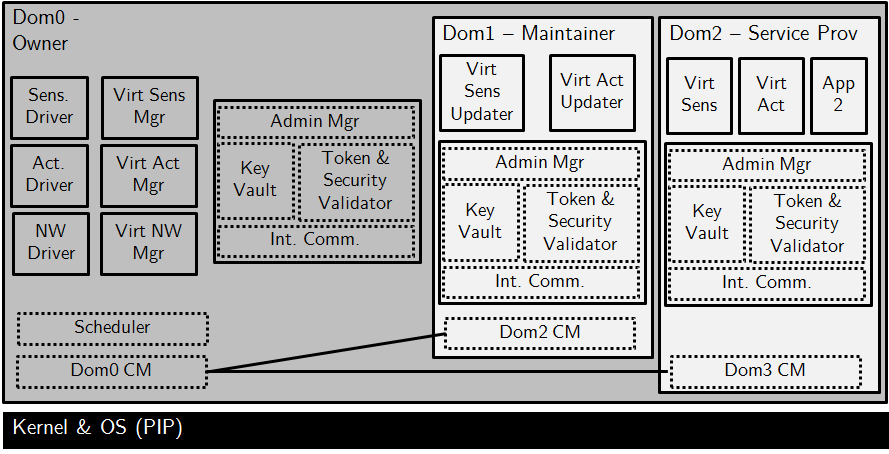
\includegraphics[width=9cm]{figures/mem_layout.png}
\caption{Proposed architecture - Memory layer view}
\label{fig:Arch_mem}
\end{figure}


\subsection{Components of a domain}
\label{sec:Domain_comp}
This section describes the role of the components which enforce the proposed security model, namely the Configuration Manager, the Administration Manager, the Token \& Security Validator and the Key Vault. The architecture proposed is also based on the use of virtual sensors and actuators.\\

Figure \ref{fig:Arch_soft} represents the software layers which correspond to the example used in figure \ref{fig:Arch_mem}. The PIP kernel exposes isolation services to an OS on which domains and partitions are created. The OS layer contains a scheduler which organizes the time and operations of the domains and partitions and each domain configuration manager. The application layer contains the drivers and all the modules of the architecture defined here. The OS and application layers both belong to user land. 

\begin{figure}[h!]
\centering
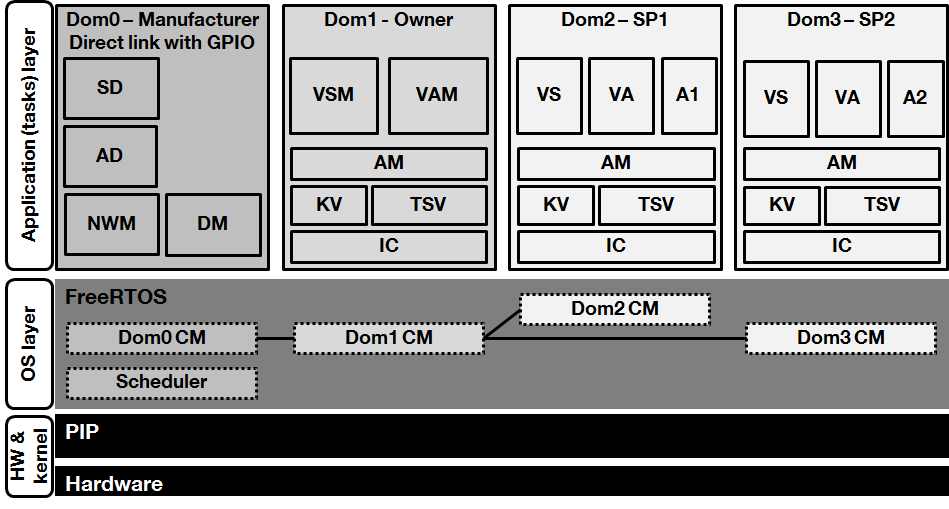
\includegraphics[width=9cm]{figures/soft_layer.png}
\caption{Proposed architecture - Software layer view}
\label{fig:Arch_soft}
\end{figure}

\subsubsection{Configuration Manager}
\label{sec:Config_Mgr}
The Configuration Manager contains a description of the domain's sub partitions, the associated code and the authorized communication channels between two partitions. It enforces the communications mechanism based on shared memory and described in section \ref{sec:Communication_model}.

\subsubsection{Internal Communicator}
\label{sec:Int_Com}
The Internal Communicator is the unique entry point of the domain. It verifies incoming messages whether they come from the network or another domain, similarly to a firewall.

\subsubsection{Virtual sensors or actuators managers}
\label{sec:virtual_sensor} 
These managers provides synthetic sensor and actuator support to the virtual sensors and actuators over the internal communication module.

\subsubsection{Virtual sensors or actuators}
\label{sec:virtual_sensor}
Only the owner domain can manage the machine-level functions such as the drivers or the physical memory. Each domain contains a virtual sensor or actuator which are a synthetic sensor or actuator instance. It consumes the hardware ressources provided by the virtual sensor or actuator manager and requires and forwards a token to the owner domain if required. This allows the entity which owns the domain to see his domain as an actual device without knowledge of the isolation. The instruction and response are transmitted to and from the real driver using the internal communication mechanism. The virtual sensor or actuator updater is specific and allows the update of the related sensor or actuator driver in the owner domain. 

\subsubsection{Administration Manager}
\label{sec:Admin_Mgr}
This module exposes the domain's ressources to an external server managed by the entity which owns the domain. It routes the command to read, write, execute the ressource to the expected manager or virtual sensor, actuator. It sends each command received to the Token \& Security Validator (T\&S Validator). 

\subsubsection{Token \& Security Validator}
\label{sec:Token_Validator}
The Token \& Security Validator (T\&S Validator) validates each device management command against the token provided in the command and optionnally an internal security policy. For example, the security policy defines which ressources require a token verification to be accessed or whether a specific command can be processed accordaccording to the device battery status. 

\subsubsection{Key Vault}
\label{sec:Key_Vault}
This module stores the keys that are used by the domain. In particular, the keys used by the Token \& Security Valdiator are stored here. It also provides the functions to add a new key, modify or delete an existing key.

\subsection{Management model}

As depicted in figure \ref{fig:Mgt_model}, the model proposed is based on master/agent model. Each domain receives commands from a server which authenticates the origin of the command and authorizes it. The administration manager in the domain is an agent which expects requests from its master, the administration application in the server. The Token \& Security Validator validates the token generated according to the access policy on the server side. For simplicity's sake, only the components \& modules related to the owner domain are detailed in figure \ref{fig:Mgt_model}.\\

\label{sec:Management_model}
\begin{figure}[h!]
\centering
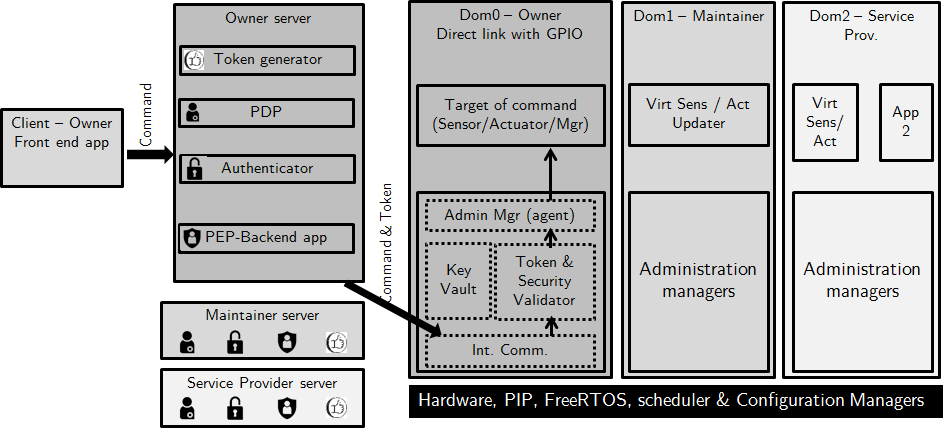
\includegraphics[width=9cm]{figures/management_model.png}
\caption{Proposed architecture - Management model}
\label{fig:Mgt_model}
\end{figure}

Each entity is responsible for managing and authorizing the access of its own domain ressources (e.g. domain token keys, application installation) to its users. The owner also manages and authorizes the access to device ressources (e.g. sensor drivers \& virtual managers) to its users and to other entities (e.g. maintainer or service provider).\\

\subsubsection{Domain ressources management}
An example is the modification of the URL from which to retrieve the package which contains a driver update. This parameter is in the perimeter of the maintainer and does not require any modification on the drivers or parameters controled by the owner. Therefore, it is the maintainer's responsiblity to ensure that this modification can be performed only by authenticated \& authorized users.\\

As illustrated in figure \ref{fig:DomRes_AP}, first, the client which requests the modification is authenticated. Then, it choses an operation proposed by the administration manager and the access policy evaluates whether this particular user is authorized to perform the selected operation. If yes, the token A is generated and the maintainer sends the command and the token are sent to the maintainer's domain where the command is processed.
\label{sec:DomRes_AP}
\begin{figure}[h!]
\centering
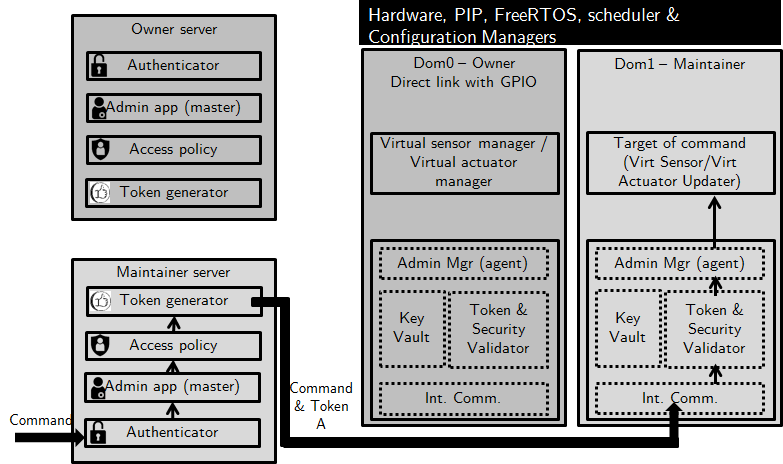
\includegraphics[width=9cm]{figures/DomRes_AP.png}
\caption{Management of domain ressources}
\label{fig:DomRes_AP}
\end{figure}

\subsubsection{Device ressources management}
An example is the download, deployment \& installation of a package with a driver udpate. In this case, the maintaier authenticates the user which requests this operation and then requests the owner the authorization to perform it.\\

Figure \ref{fig:DevRes_AP} illustrates the steps necessary for this operation. First, the client which requests the update is authenticated and authorized by the maintainer server. Then, the maintainer server forwards the request to the owner. The owner authenticates the maintainer server which initiates the request and which will deploy the update package, authorizes the operation according to its own access policy and generates token B. The maintainer server now sends the command, token A and token B to the maintainer's domain. Once token A is verified by the maintainer's Token \& Security Validator, the virtual sensor updator sends the command and token B to the Owner domain. If the owner validates token B, the update is authorized.
\label{sec:DevRes_AP}
\begin{figure}[h!]
\centering
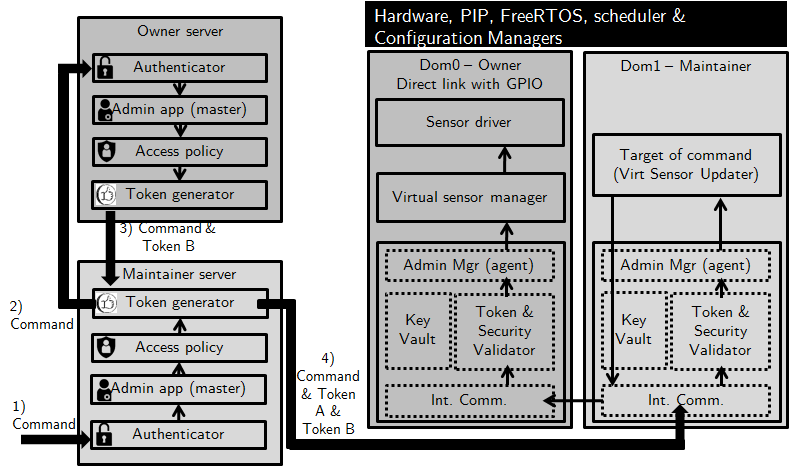
\includegraphics[width=9cm]{figures/DevRes_AP.png}
\caption{Management of device ressources}
\label{fig:DevRes_AP}
\end{figure}

\subsubsection{Token scheme}
The token format should contain at minimum a payload and a signature of this payload. Compatible token formats include JWT (JSON Web Token) \cite{rfc7519_jwt_2015} and CWT (CBOR Web Token) \cite{rfc_CWT_2017}.\\

The token's objectives are to 1) ensure that any command will reach the intended destination, 2) give the rights to request some operations on ressources, 3) prove that the entity initiating the command has been authenticated authorized and protect against replay. To achieve these goals, the token should contain at minimum:
\begin{itemize}
    \item the ID of the partition to which this token is destined,
    \item the rights granted,
    \item a proof ensuring that the token was generated by the token provider,
    \item a token ID and/or an expiration date.
\end{itemize}

The proof can either be a digital signature, such as ANS X9.31, ANS X9.62 or PKCS\#1 as recommended by NIST \cite{nist_dss_2013} or a Keyed-hash Message Authentication Codes (HMACS) compliant NIST recommendations and using a NIST-approved hash algorithm such as SHA-256 \cite{nist_hmac_2008, nist_hash_2012}, depending on the level of security and non-repudiation required.
The token ID and expiration date are used to prevent replay. The token ID can be compared to a set of previously used IDs stored in a cache. The size of the cache should be adapted to the memory constraints of the partition and device. The combination of the size of the cache and the expiration date allows achieving best effort replay detection. Therefore, it is strongly recommended to use both elements and to tune them carefully. 

\subsection{Communication model}
\label{sec:Communication_model}
%\todo[inline]{TBD. Section to be described by Lille}
The main requirement for the communication protocol is to allow master/agent communication and the transport of a payload with the command content and an associated token. Protocols such as TCP/IP or CoAP are eligible. LwM2M \cite{oma_lwm2M_2017} would require some modification to add a token to the message.

\subsubsection{Internal communication}
Each domain has an internal communication mechanism. It can be implemented by the domain itself, however, it is always based on Pip sending signal mechanism. 


\subsubsection{External communication}

For external communication, only one partition is in charge of Network hardware sending and receiving functions. In order to send a external message, each domains has to use the internal communication to discuss with the Network manager, and send it the external message. 
%\lipsum[1-6]



%The aim of ODSI and PIP is to provide an isolation which allows multiple applications to coexist he aim of ODSI architecture is to provide a safe environment for each service provider. In other words, the aim of ODSI and Pip is to preserve the trust between each service provider and between the platform and the service provider.  
%\subsection{Trust between service providers}

%Each service provider has to trust the platform and the platform has to guarantee to each 

%\todo[inline]{TOD0: 
%- Confiance entre service, chaque service doit se voir garantir que son �tat ne peut �tre alt�r� par un autre service, potentiellement concurent

%- Chaque service doit faire confiance � la platforme, �tant donn�e qu'elle est dans sa TCB.}


%\subsection{Need in separation}

%\todo[inline]{TOD0: 
%	- Pip fournit l'isolation recherch�e par les services pour garantir leur espace de travail/ espace d'adressage
%	- Le m�chanisme de token garantit que chaque service ne peut �tre acc�d� que via l'API qu'il aura expos� et sans plus}

\section{Illustration \& discussion}

\label{sec:illustration_discussion}
\subsection{Pip and ODSI architecture}

The ODSI architecture can be build using Pip partition creation mechanism (figure \ref{fig:odsiplatformebypip}). The Owner is the first domain created and it is Pip root partition. For each sensitive component, a dedicated partition is created (Hardware Drivers, Administration manager). The Maintainer domain is also into a partition in order to give the owner the ability to limit the maintainer's rights. Each other services has also to be into partition, because we need to isolate them from any threat or data leak, only the Owner can access to them.



\begin{figure}[ht]
	\centering
	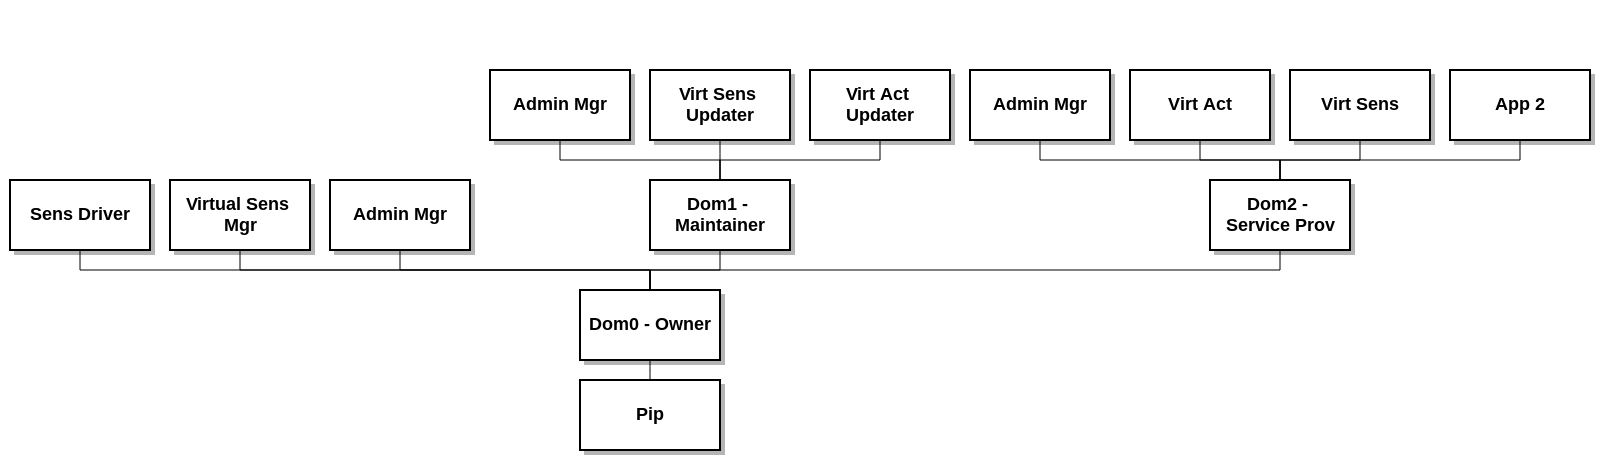
\includegraphics[width=1\linewidth]{figures/ODSIPlatformeByPip}
	\caption{ODSI platform build with Pip partition tree}
	\label{fig:odsiplatformebypip}
\end{figure}



%\todo[inline]{TBD. Section to show how the isolation model allows to address the industrial needs}

An example of application of the proposed architecture is illustrated in figures \ref{fig:houseiot}, \ref{fig:ODSIGateway} and \ref{fig:ODSIDevice}. One or several home smart devices are associated to a domain in the gateway, \ref{fig:houseiot}. Each domain in the gateway exposes the associated small devices ressources to the outside worlds \ref{fig:ODSIGateway}. The devices are managed by only one entity and contains only one domain. Several partitions are created to isolate functions of the device.\\

As depicted in figure \ref{fig:ODSIGateway}, domain 1 is managed by an audiovisual Service Provider which proposes an application to control a connected TV and audio device. Domain 2 is managed by an electronic device management which proposes an application to control a game console, electric outlets and connected lamps. These applications forward the commands and their token to the associated devices. The authentication and token generation can be done by the a service in the domain (e.g. domain 2) or by a service in the cloud (e.g. domain1). The NAT functionality is also isolated from other services in the gateway. Similary to small devices, all applications the three domains perform actions only if they are authenticated and authorized by a token issued by an application in the cloud.\\

As depicted in figure \ref{fig:ODSIDevice}, small devices only have one domain and several isolated functionalities. For example, network drivers which are a potential entry point for attacks are isolated from other drivers and applications in the device. 

\begin{figure}[h]
	\centering
	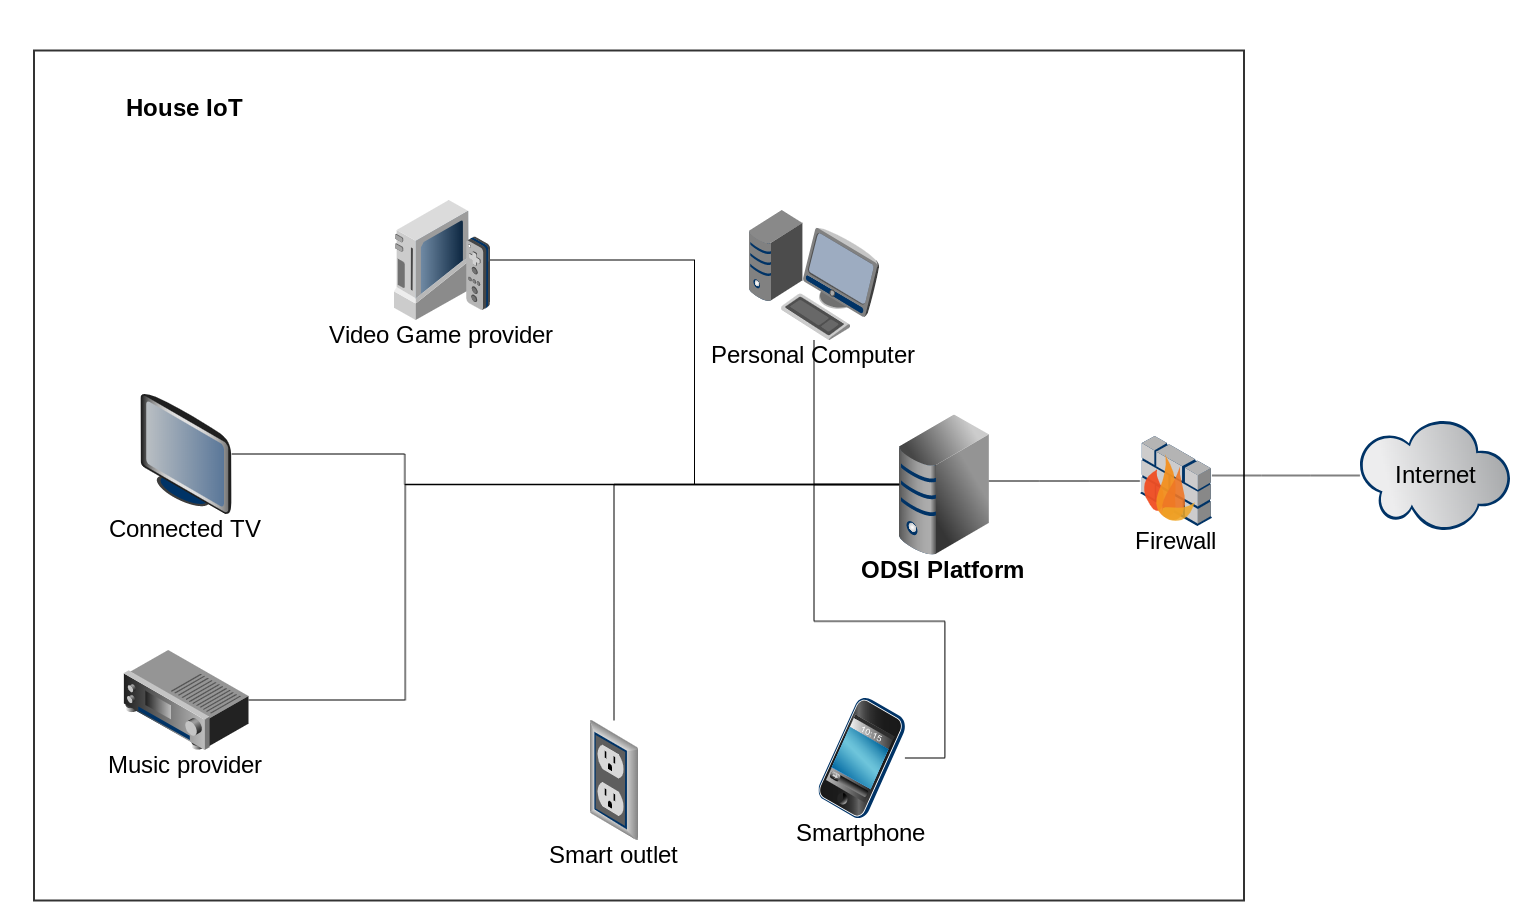
\includegraphics[width=1\linewidth]{figures/HouseIOT}
	\caption[House IoT installation example]{House IoT installation example}
	\label{fig:houseiot}
\end{figure}
\begin{figure}[h]
	\centering
	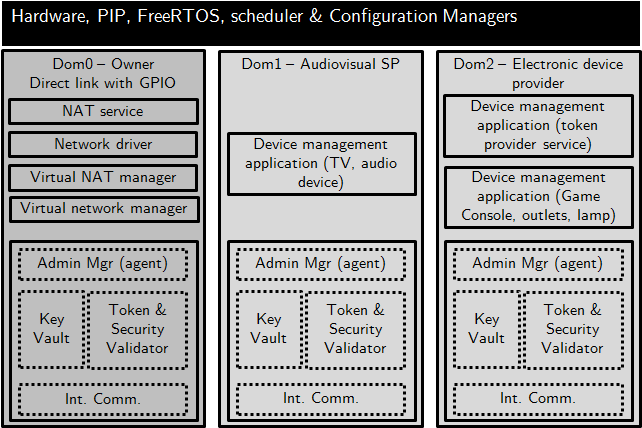
\includegraphics[width=1\linewidth]{figures/ODSIGateway}
	\caption{ODSI Gateway}
	\label{fig:ODSIGateway}
\end{figure}
\begin{figure}[ht]
	\centering
	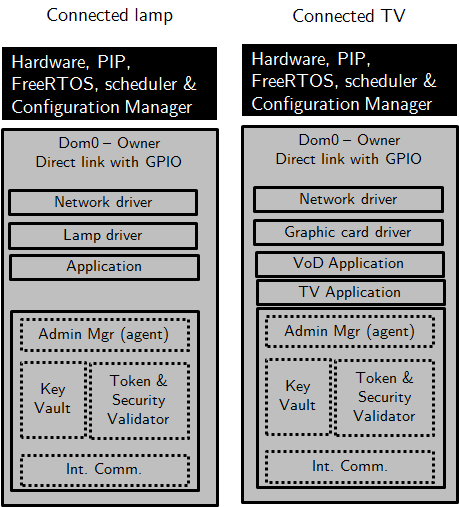
\includegraphics[width=0.6\linewidth]{figures/ODSIDevice}
	\caption{Two examples of smart home devices (connected lamp and connected TV)}
	\label{fig:ODSIDevice}
\end{figure}

The proposed security architecture avoids the attack described by Sivaraman et.al.\cite{Sivaraman2016}. Indeed, the token mechanism is used to authenticate each command sent to the devices or to the NAT configuration service in the router.\\

Using Pip enhances the protection against this attack by creating isolated partitions in the router and in the devices. Therefore, a successful attack against a domain in the gateway or a partition in the home smart devices can be contained. \\

%\lipsum[1-4]

\section{Conclusion}
%\todo[inline]{TBD. The conclusion goes here. Next steps : implementation and performance evaluation}
%\lipsum[1-2]
In this paper we have described an architecture based on a separation kernel in order to provide a trustworthy environment for multiple economic competitors into the same IoT device. This architecture is defined by a set of actors which each one is limited into its capabilities, depending on its role into the platform. By using the separation kernel Pip, we can provide security and safety guarantees between each actor into the device. The Token mechanism used into the platform guarantee all external and internal communication for the IoT device. 


% conference papers do not normally have an appendix


% use section* for acknowledgment
\section*{Acknowledgment}
This article was done in the scope of the European Celtic-Plus project ODSI.  





% trigger a \newpage just before the given reference
% number - used to balance the columns on the last page
% adjust value as needed - may need to be readjusted if
% the document is modified later
%\IEEEtriggeratref{8}
% The "triggered" command can be changed if desired:
%\IEEEtriggercmd{\enlargethispage{-5in}}

% references section

% can use a bibliography generated by BibTeX as a .bbl file
% BibTeX documentation can be easily obtained at:
% http://mirror.ctan.org/biblio/bibtex/contrib/doc/
% The IEEEtran BibTeX style support page is at:
% http://www.michaelshell.org/tex/ieeetran/bibtex/
%\bibliographystyle{IEEEtran}
% argument is your BibTeX string definitions and bibliography database(s)
%\bibliography{IEEEabrv,../bib/paper}
%
% <OR> manually copy in the resultant .bbl file
% set second argument of \begin to the number of references
% (used to reserve space for the reference number labels box)

% An example of a floating figure using the graphicx package.
% Note that \label must occur AFTER (or within) \caption.
% For figures, \caption should occur after the \includegraphics.
% Note that IEEEtran v1.7 and later has special internal code that
% is designed to preserve the operation of \label within \caption
% even when the captionsoff option is in effect. However, because
% of issues like this, it may be the safest practice to put all your
% \label just after \caption rather than within \caption{}.
%
% Reminder: the "draftcls" or "draftclsnofoot", not "draft", class
% option should be used if it is desired that the figures are to be
% displayed while in draft mode.
%
%\begin{figure}[!t]
%\centering
%\includegraphics[width=2.5in]{myfigure}
% where an .eps filename suffix will be assumed under latex, 
% and a .pdf suffix will be assumed for pdflatex; or what has been declared
% via \DeclareGraphicsExtensions.
%\caption{Simulation results for the network.}
%\label{fig_sim}
%\end{figure}

% Note that the IEEE typically puts floats only at the top, even when this
% results in a large percentage of a column being occupied by floats.


% An example of a double column floating figure using two subfigures.
% (The subfig.sty package must be loaded for this to work.)
% The subfigure \label commands are set within each subfloat command,
% and the \label for the overall figure must come after \caption.
% \hfil is used as a separator to get equal spacing.
% Watch out that the combined width of all the subfigures on a 
% line do not exceed the text width or a line break will occur.
%
%\begin{figure*}[!t]
%\centering
%\subfloat[Case I]{\includegraphics[width=2.5in]{box}%
%\label{fig_first_case}}
%\hfil
%\subfloat[Case II]{\includegraphics[width=2.5in]{box}%
%\label{fig_second_case}}
%\caption{Simulation results for the network.}
%\label{fig_sim}
%\end{figure*}
%
% Note that often IEEE papers with subfigures do not employ subfigure
% captions (using the optional argument to \subfloat[]), but instead will
% reference/describe all of them (a), (b), etc., within the main caption.
% Be aware that for subfig.sty to generate the (a), (b), etc., subfigure
% labels, the optional argument to \subfloat must be present. If a
% subcaption is not desired, just leave its contents blank,
% e.g., \subfloat[].

\bibliographystyle{unsrt}
\bibliography{biblio}





% that's all folks
\end{document}


